\chapter{绪论}
\section{研究背景及意义}
随着现代战争形态的日益演变,无人机正逐渐成为战场上的关键因素。特别的,在战场环境日益复杂且不可预测的背景下,垂直起降无人机引起了广泛的关
注,特别注意的是学术上所提及的垂直起降一般指垂直起降固定翼飞行器而非直升机及多旋翼类无人机。这是因为相较于传统固定翼无人机,其能在无需跑道的条件下完成自主起飞与
降落。此外,区别于多旋翼无人机以多个旋翼提供升力的飞行方式,垂直起降无人机依靠机翼产生升力,从而提供更大的有效载荷容量、更快的巡航速度和更远的飞行距离\cite{okulski2022small}。

%广义上,直升机及多旋翼无人机也具备垂直起降能力,但本文提及的垂直起降飞行器一般指垂直起降固定翼飞行器。
通常来说,垂直起降无人机具备两种典型工作状态,分别是垂直起降模态和水平飞行模态,根据两种模态转换方式的特点,垂直起降无人机可大致分为倾转式无人机、复合式无人机
和尾座式无人机,其中,尾座式是一种的独特的垂直起降飞行器,其在垂直起降阶段保持机头朝上,机身竖立,并依靠尾部大推力发动机产生推力抵消重力,
并通过在空中倾转姿态完成垂直与水平模态间的转换过程(又称过渡模态)。与倾转式或复合式垂直起降飞行器相比,尾座式没有任何冗余的垂直起降机构,具备结构简单、可靠性高的
优点,尤其适合在军事领域中进行侦察、打击、补给、通讯中继和在民用领域中进行监控、搜索等。

近年来,出现了一种新型的尾座式飞行器,其采用涵道风扇作为尾部的单一矢量动力单元,保证了无人机在极端恶劣条件下的控制能力,此外,涵道的构型可以提升同等功率下发动机的
推力从而提高无人机有效载荷质量,同时还可以减轻工作噪声以及保证操作人员的安全性。更为重要的是,由于涵道风扇的存在,涵道风扇尾座式无人机(Duted-fan Tail-sitter Unmanned Aerial Vehicles,简称DFTSUAV)
拥有更强的低速、大迎角姿态控制能力,为无人机完成各种复杂的机动任务提供了可行性。

DFTSUAV具备两种工作模态,分别是垂直悬停模态(Hover)与水平飞行模态(Level flight)以及对应的两种过渡模态即垂直悬停到水平飞行(Hover To Level flgiht,HTL)的过渡过程和
水平飞行到垂直悬停(Level flgiht To Hover,LTH)的逆过渡过程。DFTSUAV在悬停模态和水平飞行模态下通常可以参照传统多旋翼与固定翼的控制方法进行设计,而在过渡模态下由于无人
机工作平衡点的变化和大攻角(Angle of Attack,AoA)所引发的失速现象,DFTSUAV的飞行动力学呈现很强的非线性、多模态和强耦合特性。尤其是在逆过渡过程中,飞行器往往会进入不可控
的稳态从而过渡失败变回初始悬停状态,因此研究一种快速稳定的逆过渡控制策略对于涵道风扇尾座式无人机具有重要的意义。


\section{国内外研究现状}
\subection{涵道风扇尾座式飞行器研究现状}
然而,目前这类无人机的成功研制案例较少,仅包括:美国Shield-AI公司的V-bat,韩国KAIST实验室与中国华南理工大学。
\subection{过渡控制方法研究现状}
众所周知,涵道风扇式垂直起降无人机具备两种典型的工作
模态分别是:水平飞行模态(level flgiht)和垂直悬停模态(hover)。逆过渡(Back-transition)问题的目标主要是实现由水平飞行模态转垂直悬停模态即(Level flight to Hover,LTH),也
是被认为难度较大的过渡过程。

最简单直接的逆过渡策略就是令无人机以一个较大的俯仰角爬升\cite{green2005mav},将无人机水平飞行的动能转化为重力势能,例如:开源飞控“PX4”中以恒定油门和阶跃俯仰角信号为输入的线性
过渡轨迹和\cite{jeong2010transition}中提到的连续上升轨迹。在这种只强调能否完成逆过渡的方法基础上,过渡过程中的性能表现也逐渐被人们关注,例如:过渡转换时间,过渡过程高度变化,
过渡过程飞行距离
等。传统的过渡控制策略通常要求在先验给出参考过渡轨迹的条件下再去设计
控制器去进行跟踪。轨迹优化则通过直接法或间接法去求解一个最优控制问题来求解相应的过渡控制策略。
\subection{强化学习研究现状}

\section{研究内容与主要贡献}
\section{论文组织结构}

\chapter{涵道风扇式无人机数学模型与强化学习基础知识}
\section{引言}
本章主要对过渡过程中涵道风扇无人机数学模型以及强化学习的相关知识进行简要概述。涵道风扇式无人机在实现过渡过程中,其飞行姿态会发生
剧烈的变化,因此建立一个能够精准地描述其非线性特性的仿真数学模型是设计过渡策略的前提。本章首先介绍了描述无人机运动所需要的坐标系
及运动参数,然后详细介绍了涵道风扇式无人机的结构,并针对涵道风扇式无人机的每个关键模块介绍其物理机理,然后基于牛顿-欧拉方法并结合
动力学与运动学方程建立涵道风扇式无人机六自由度数学模型,最后介绍了强化学习的相关知识包括其基本概念,然后分别介绍了同策略强化学习和
异策略强化学习,为后续强化学习算法设计奠定了基础。

\section{坐标系及其变换}
\subsection{常用坐标系与无人机运动参数}
\label{sec:1}
无人机的六自由度运动包括平移和旋转运动,为方便描述无人机的运动状态,引入如下坐标系:
\begin{figure}[htbp]
    \centering
    \begin{minipage}{.49\linewidth}
        \centering
        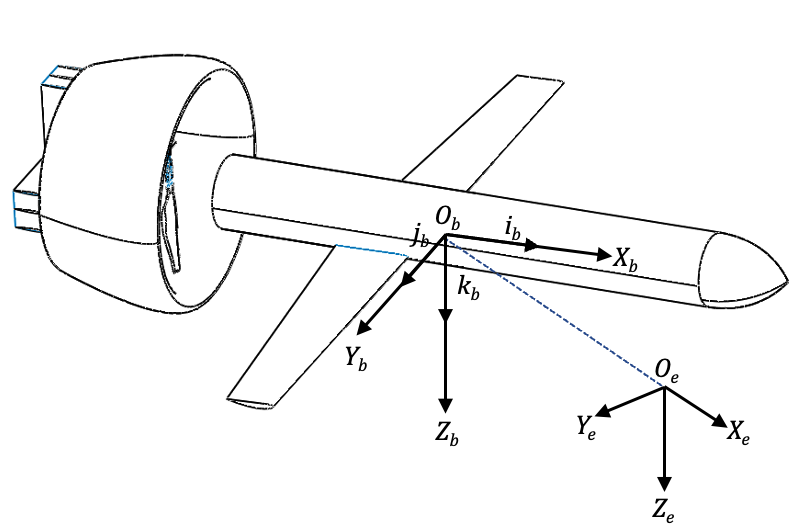
\includegraphics[width=\linewidth]{coordinate.png}
        \caption{地面坐标系及机体坐标系}
        \label{fig:coordinate}
    \end{minipage}
    \hfill
    \begin{minipage}{.49\linewidth}
        \centering
        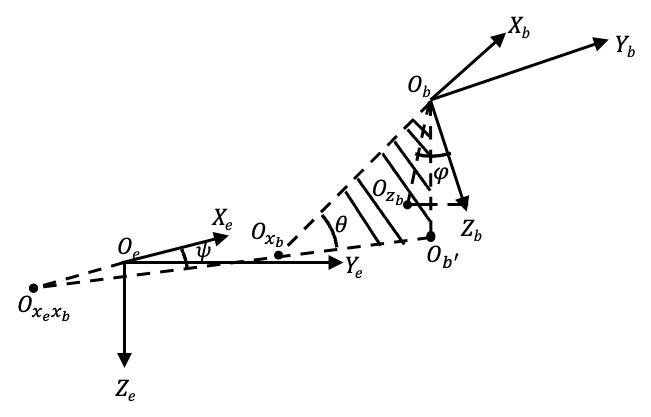
\includegraphics[width=\linewidth]{euler.png}
        \caption{欧拉角}
        \label{fig:euler}
    \end{minipage}
\end{figure}

\begin{itemize}
\item [1.] 
    地面坐标系:地面坐标系$o_{e}x_{e}y_{e}z_{e}$定义为与地球表面固连的坐标系,通常用于研究无人机相对于地面的运动状态,确定机体的三维位置,忽略地球曲率,即将地球表面假设
    成平面。通常以无人机起飞位置作为坐标原点$o_{e}$,先让$o_{e}x_{e}$轴在水平面内指向某一方向,$o_{e}z_{e}$轴垂直与地面向下,然后以右手定则确定$o_{e}y_{e}$轴。       
\item [2.]
    机体坐标系:机体坐标系$o_{b}x_{b}y_{b}z_{b}$与无人机机体固连。其原点$o_{b}$选取在无人机质心上;$o_{b}x_{b}$轴在无人机对称平面内沿机身轴线指向前方;
    $o_{b}z_{b}$在无人机对称平面内,垂直于$o_{b}x_{b}$轴向下,然后可以以右手定则确定$o_{b}y_{b}$。机体坐标系与地面坐标系的关系如\autoref{fig:coordinate}所示。

    机体坐标系相对于地面坐标系的方位,或者说无人机在空中的姿态,通常可以用三个欧拉角表示,分别是俯仰角$\theta$、滚转角$\phi$、偏航角$\psi$,如\autoref{fig:euler}所示。
    图中$o_{b^{'}}$表示$o_{b}$在平面$o_{e}x_{e}y_{e}z_{e}$上的投影,$o_{x_{b}}$表示$x_{b}o_{b}$延长线与平面$o_{e}x_{e}y_{e}$的交点,$o_{b}o_{z_{b}}$表示
    $o_{b}z_{b}$在通过机体轴$o_{b}x_{b}$的铅锤面$o_{b}o_{x_{b}}o_{b^{'}}$上的投影;$o_{x_{e}x_{b}}$表示$x_{e}o_{e}$延长线与$o_{b^{'}}o_{x_{b}}$延长线的交点。

    其中,俯仰角$\theta$即是$o_{b}x_{b}$轴与平面$o_{e}x_{e}y_{e}z_{e}$的夹角,如果$o_{b}x_{b}$轴指向上方为正,否则为负。俯仰角实质上是描述无人机相对低面
    低头或抬头程度的物理量。

    滚转角$\phi$即是$o_{b}z_{b}$轴与铅锤面$o_{b}o_{x_{b}}o_{b^{'}}$之间的夹角,取$o_{b}z_{b}$轴指向铅锤面$o_{b}o_{x_{b}}o_{b^{'}}$的左方为正,
    否则为负。滚转角实质上是描述无人机绕其纵轴滚转程度的物理量。

    偏航角$\psi$即是$o_{b}x_{b}$轴在平面$o_{e}x_{e}y_{e}z_{e}$上的投影与$o_{e}x_{e}$延长线的夹角。取地面坐标系顺时针转动为正,否则为负。偏航角实质上是
    描述无人机偏离航线程度的物理量。

\item [3.]
气流坐标系:气流坐标系$ox_{a}y_{a}z_{a}$定义为与机体固连的坐标系。原点$o$固定在无人机的瞬时质心伤;$ox_{a}$轴与无人机速度矢量$V_{a}$重合,$oz_{a}$轴位于无人机对称平面
内,垂直于$ox_{a}$轴指向下方;然后可以以右手定则确定$oy_{a}$轴,无人机的气动力在气流坐标系下很容易表示,因此,通常需要使用攻角$\alpha$和侧滑角$\beta$来进行气流坐标系与机
体坐标系下的转换,如\autoref{fig:stabilityframe}所示。攻角$\alpha$定义为飞行速度矢量$V_{a}$在无人机对称平面上的投影与机体轴$ox_{b}$之间的夹角。侧滑角$\beta$定义为飞
行速度矢量$V_{a}$与无人机对称平面之间的夹角。
\end{itemize}
\begin{figure}[htbp]
    \centering
    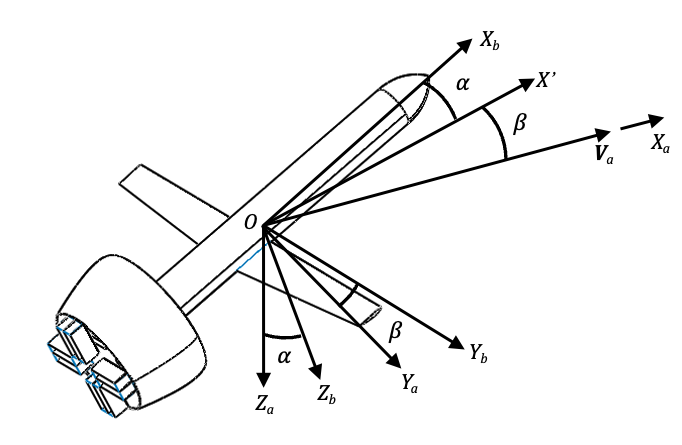
\includegraphics[width=0.5\textwidth]{stabilityframe.png}
    \caption{\label{fig:stabilityframe}气流坐标系与机体坐标系}
\end{figure}
\subsection{坐标变换}
在建立无人机运动方程前,还需要知道各坐标系之间的相互投影关系,即坐标转换矩阵。
\begin{itemize}
\item [1.] 地面坐标系与机体坐标系间的变换:\\
在无人机在飞行过程中,地面坐标系能确定的仅仅是无人机质心在任意时刻相对于地面的位置,而无法确定无人机相对于地面的姿态。
而常见的姿态表示方法包括:欧拉角、旋转矩阵和四元数,其中,
欧拉角是一种具有直观和简便的几何意义的姿态表示方式,定义如\autoref{sec:1}中所述。而根据欧拉定理,刚体绕固定点的旋转可以看作是若干次有限有限旋转的合成。在欧拉转动中,地面坐标系转动三次即可
得到机体坐标系。在这三次旋转中,旋转轴是待转动坐标系的某一对应坐标轴,旋转角度即为欧拉角。在传统的“$ZYX$”旋转顺序下,欧拉角在$90^\circ$俯仰角时会存在奇异的情况,而
无人机的过渡过程通常要求俯仰角变化$90^\circ$同时滚转角变化较小。
因此本文采用了“$ZXY$”旋转顺序定义的欧拉角,在该定义下,俯仰角的取值范围扩充至$\left [ -180^\circ,180^\circ \right ]$,
奇异点变成了$90^\circ$滚转角,有效避免了俯仰运动的奇异性。对于“$ZXY$”旋转顺序,每次旋转的角度依次为:$\psi$(偏航角)、$\phi$(滚转角)、$\theta$(俯仰角),绕各种转动的坐标
转换矩阵分别如下:
\begin{align}
    R_{z}(\psi) & = \begin{bmatrix}
      \cos\psi&  -\sin\psi& 0\\
      \sin\psi&  \cos\psi& 0\\
      0&  0& 1
    \end{bmatrix}\\
    R_{x}(\phi) & = \begin{bmatrix}
      1&  0& 0\\
      0&  \cos\phi& -\sin\phi\\
      0&  \sin\phi& \cos\phi
    \end{bmatrix}\\
    R_{y}(\theta) & = \begin{bmatrix}
      \cos\theta&  0& \sin\theta\\
      0&  1& 0\\
      -\sin\theta&  0& \cos\theta
    \end{bmatrix}
\end{align}
由此可得"$ZXY$"旋转顺序下由机体坐标系到地面坐标系的旋转矩阵$R_{b}^{e}$:
\begin{align}
    R_{b}^{e} &= R_{z}(\psi)R_{x}(\phi)R_{y}(\theta) \nonumber \\
    &= \begin{bmatrix}
     \cos \theta\cos \psi -\sin \phi \sin \theta \sin \psi&  -\sin\psi\cos\phi& \cos\psi\sin\theta+\sin\psi\sin\phi\cos\theta  \\
     \sin\psi\cos\theta+\cos\psi\sin\phi\sin\theta&  \cos\psi\cos\phi& \sin\psi\sin\theta-\cos\psi\sin\phi\cos\theta\\
      -\cos\phi\sin\theta&  \sin\phi& \cos\phi\cos\theta
    \end{bmatrix}
\end{align}
\item [2.] 气流坐标系与机体坐标系间的变换:\\
由气流坐标系定义可知,机体坐标系与气流坐标系之间的关系可以只用攻角和侧滑角来描述,也就是说气流坐标系只要旋转两次即可得到机体坐标系。即:
\begin{align}
    L(\alpha)&=
    \begin{bmatrix}
      \cos\alpha&  0& -\sin\alpha\\
      0&  1& 0\\
      \sin\alpha &  0& \cos\alpha 
    \end{bmatrix} \\
    L(\beta)&=
    \begin{bmatrix}
      \cos\beta&  \sin\beta& 0\\
      -\sin\beta&  \cos\beta& 0\\
      0 &  0& 1 
    \end{bmatrix}
\end{align}
由此可得气流坐标系到机体坐标系的转换矩阵为:
\begin{align}
    L_{a}^{b}&= L(\alpha)L(\beta) \nonumber \\
    &=
    \begin{bmatrix}
      \cos\alpha\cos\beta&  \cos\alpha\sin\beta& -\sin\alpha\\
      -\sin\beta&  \cos\beta& 0\\
      \sin\alpha\cos\beta &  \sin\alpha\sin\beta& \cos\alpha 
    \end{bmatrix} 
    \label{eq:Lab}
\end{align}
\end{itemize}                                         
\section{无人机运动学模型}
运动学与质量与受力无关,只研究无人机位置、速度、姿态和角速度等变量。通常情况下,运动学模型的输入为速度和角速度,输出为位置和姿态。
在刚体假设下,无人机六自由度运动学方程可以由质点的运动学方程和欧拉运动学方程描述,分别为:
\begin{equation}
    \left\{\begin{array}{l}
        {\dot{\mathbf{p}}}^{e}={\mathbf{v}}^{e} \\
        \dot{\mathbf{\Theta}}=\mathbf{Q} {\mathbf{\omega}}^{b} \\
        \end{array}\right.
\end{equation}
其中,$\mathbf{p}$表示为无人机的位置向量,$\mathbf{v}^{b}$表示无人机在机体坐标系下的速度,$\mathbf{\Theta}$为无人机的欧拉角,${\mathbf{\omega}}^{b}$表示无人机的角速度,在$ZXY$旋转顺序下
描述欧拉角变化率与角速度关系的$\mathbf{Q}$如下定义:
\begin{equation}
    \mathbf{Q} \triangleq\left[\begin{array}{ccc}
        \cos\theta & 0 & \sin\theta \\
        \sin\theta\tan\varphi  & 1 & -\cos\theta\tan\varphi  \\
        -\sin\theta/\cos\varphi  & 0 & \cos\theta/ \cos\varphi
        \end{array}\right]
\end{equation}
\section{无人机动力学模型}
动力学既涉及运动又涉及无人机受力情况,与无人机的质量与转动惯量有关,动力学模型的输入为合外力与合外力矩
,输出为速度与角速度。无人机动力学模型与运动学模型一起构成了无人机飞行控制刚体六自由度模型。
\begin{figure}[htbp]
    \centering
    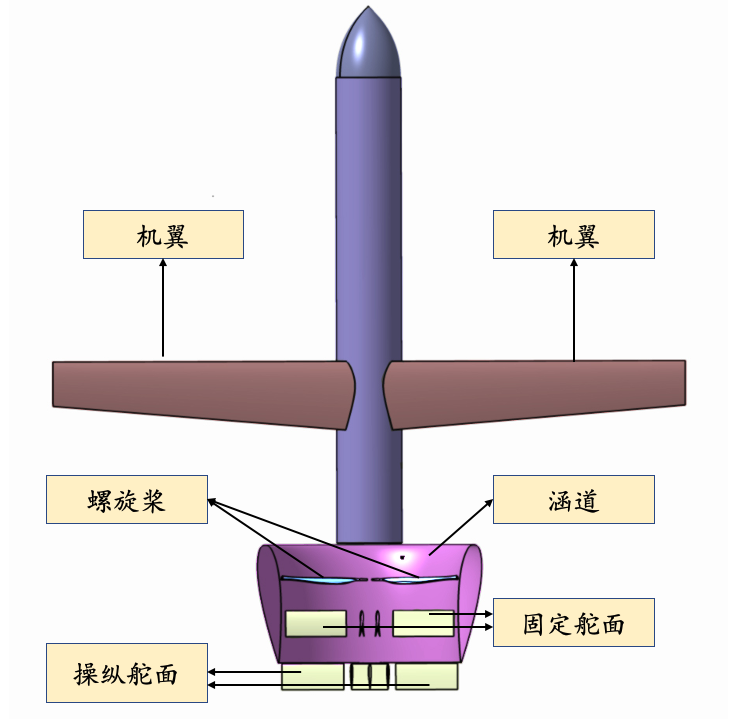
\includegraphics[width=0.4\textwidth]{wholebody.png}
    \caption{\label{fig:layout}涵道风扇式无人机总体结构图}
\end{figure}

涵道风扇式无人机可以认为主要由五个不同的子模块构成,如\autoref{fig:layout}所示,分别是:
一、涵道螺旋桨:涵道螺旋桨主要负责为无人机提供推力,是无人机悬停状态下的动力来源,其产生的诱导速度同时也会影响到舵面的操纵效率;
二、涵道:涵道为环形机翼结构,因此涵道机身本身上也会产生一定的气动力,同时由于涵道对于气流的对齐作用,涵道还会受侧风影响产生一
定的动量阻力与动量阻力矩,此外还可以减少气流损失,提高螺旋桨的气动效率;
三、操纵舵面:涵道无人机的涵道内部有四组独立偏转的操纵舵面,每组操纵舵面由三片带有翼型的矩形舵板组成,涵道下洗气流流经操纵舵面产生气动
力和气动力矩,因此通过操纵四组舵面的偏转就可以改变无人机的运动状态;
四、机翼及机身:机翼与机身会产生气动力及其产生的力矩,这也是无人机水平飞行状态下的动力来源;
五、固定舵面:固定舵面主要用来平衡悬停状态下螺旋桨产生的反扭距,提高悬停效率。
因此,定义合力$\mathbf{F}$和合力矩$\mathbf{M}$如下:
\begin{align}
    \mathbf{F} & =\mathbf{F}_{prop}+\mathbf{F}_{aero}+\mathbf{F}_{cs}+\mathbf{F}_{d}\\
    \mathbf{M} & =\mathbf{M}_{aero}+\mathbf{M}_{prop}+\mathbf{M}_{gyro}+\mathbf{M}_{cs}+\mathbf{M}_{d}+\mathbf{M}_{f}
\end{align}
其中,$\mathbf{F}_{prop}$和$\mathbf{M}_{prop}$表示涵道内部螺旋桨产生的推力与反扭力矩,
$\mathbf{F}_{aero}$和$\mathbf{M}_{aero}$表示机翼与机身上所产生的气动力和气动力矩,
$\mathbf{F}_{cs}$和$\mathbf{M}_{cs}$表示涵道底部的操纵舵面舵产生的力和力矩,
$\mathbf{F}_{d}$和$\mathbf{M}_{d}$表示涵道机身上所受到的力和力矩,
$\mathbf{M}_{f}$表示固定舵面产生的力矩,$\mathbf{M}_{gyro}$表示无人机的陀螺力矩。

综上,结合运动学和动力学模型,可得无人机六自由度运动方程为:
\begin{align}
\left\{\begin{array}{l}
    \dot{\mathbf{p}}^{e}=\mathbf{v}^{e} \\
    \dot{\mathbf{v}}^{e}=\mathbf{R}_{\mathrm{b}}^{e} \mathbf{F}+g\mathbf{e}_{3} \\
    \dot{\mathbf{\Theta}}=\mathbf{Q} {\mathbf{\omega}}^{b} \\
    \dot{\mathbf{\omega}}^{b}=\mathbf{M}+\mathbf{J}^{-1}\left(\mathbf{J} {\mathbf{\omega}}^{b} \times {\mathbf{\omega}}^{b}\right)
    \end{array}\right.
\end{align}
其中,$g$表示重力加速度,$\mathbf{e}_{3}$为地面坐标系下$Z_{e}$轴的单位向量,$\mathbf{J}$表示转动惯量矩阵,接下来会给出
相应模块的机理及具体表达式。
\subsection{涵道螺旋桨动力学}
涵道风扇式无人机的螺旋桨动力学模型极为复杂。在模拟其产生的推力时,有多种理论和方法可供选择。大多数方法在计算过程中都假设了诱导速度是已知的,
或对流场中的空速和螺旋桨的相对方向施加了严格的约束条件。然而,一种结合了基本动量理论和叶素理论的模型,最初是为具有较大展弦比的直升机旋翼设
计的,现已成功应用于涵道风扇式无人机的螺旋桨模拟。Johnson 等人已经证明,尽管在构建此模型时没有考虑涵道中的不稳定流动,该模型仍能为涵道
风扇中的螺旋桨提供相当精确的模拟效果\cite{johnson2006modeling}。螺旋桨的推力和气流速度受到沿机体轴$X_{b}$的气流方向、螺旋桨的角速度以及
螺旋桨叶片的几何形状的影响,公式如下\cite{choi2012static}:
\begin{align}
    v_{b} &= \left ( u-u_{wind} \right )  + \frac{2}{3}\omega_{p}r_{p}\left ( \frac{3}{4}K_{twist}\right )\\
    T &= \frac{1+k_{aug}}{4} \left ( v_{b}-v_{i}  \right )\omega _{p}r_{p}^{2}\rho _{\infty}a_{0}bc_{p}   
\end{align}
式中,$v_{b}$表示通过螺旋桨的气流速度,$T$表示螺旋桨产生的推力,$v_{i}$表示诱导速度, $\omega_{p}$表示螺旋桨的旋转角速度, $r_{p}$表示螺旋桨的
半径,$k_{twist}$表示叶片的扭转系数,$a_{0}$表示螺旋桨旋翼叶片升力曲线斜率,$b$表示叶片个数, $c_{p}$表示螺旋桨叶片弦长, $\rho _{\infty}$
表示空气密度, $\mathbf{v}^{b}=\left [ u,v,w \right ]^{T}$表示无人机体轴下的速度,$\mathbf{v}_{wind}=\left [ u_{wind},v_{wind},w_{wind} \right ]^{T}$
表示沿机体轴的风速。

此外,涵道还会提升螺旋桨一定的气动效率。基于Horn的理论\cite{myers2009aerodynamic},涵道对于螺旋桨所产生的影响可以用$K_{aug}$来表示,
这是一个可以描述涵道对于螺旋桨的增升作用\cite{杜思亮2016轴流状态下涵道螺旋桨增升方法的数值模拟}的比例系数,$0<= k_{aug}<= 1$,当它为1时,
表示理想状态下涵道的存在可以令螺旋桨多产生一倍的推力,当它为0时,可以被认为此时不存在涵道,推力的产生只取决于螺旋桨本身。

涵道在涵道末端远场速度$v_{f}$和诱导速度$v_{i}$可以被表示为
\begin{align}
    v_{f}&=\sqrt{\left ( u-u_{wind}+v_{i}  \right )^{2}+\left (  w - w_{wind}\right ) ^{2}+\left ( v - v_{wind}\right )^{2}} \\
    v_{i}&=\frac{T}{2\rho _{\infty}\pi r_{p}^2v_{f}} 
\end{align}
显而易见的是,上面描述螺旋桨推力以及诱导速度的公式并不存在一个闭式解析解。因此针对这个非线性耦合代数方程组(2-3)-(2-6),可以采取牛顿-拉夫逊算法进行迭代求解。
\begin{align}
    f\left(v_{i}\right)=v_{i}-\frac{\frac{1+k_{aug}}{4} \left(v_{b}-v_{i}\right) \omega _{p}r_{p}^{2}\rho _{\infty}a_{0}bc_{p}}{2 \rho _{\infty} \pi\left(\sqrt{\left ( u-u_{wind}+v_{i}  \right )^{2}+\left (  w - w_{wind}\right ) ^{2}+\left ( v - v_{wind}\right )^{2}}\right.}
\end{align}
在提供足够合理的初值下,通过牛顿-拉夫逊算法可以对螺旋桨推力以及诱导速度进行求解。因此螺旋桨产生的推力可写成如下形式:
\begin{align}
    \mathbf{F}_{\text {prop}}=\left[\begin{array}{c}
        T \\
        0 \\
        0
        \end{array}\right]
\end{align}
作用在旋翼上的电机功率可由下方公式计算得出\cite{任小璐2014涵道式无人飞行器建模与控制方法研究}:
\begin{align}
    P_{ind}=\frac{v_{i} T}{1+k_{aug}}
\end{align}
空气作用在旋翼上而产生的反扭力矩可表示为:
\begin{align}
    \mathbf{M}_{\text {prop}}=\left[\begin{array}{lll}
        \frac{P_{ind}}{\omega_{p}} & 0 & 0
        \end{array}\right]^{T}
\end{align}

\subsection{涵道空气动力学}
\begin{figure}[htbp]
    \centering
    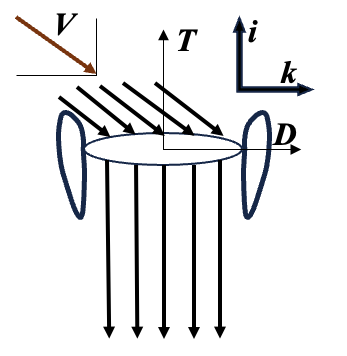
\includegraphics[width=.3\linewidth]{momentum.png}
    \caption{\label{fig:momentum}动量阻力示意图}
\end{figure}
通常情况下,涵道一般会被视为是无人机升力体的一部分,并不会单独建模其作为环形机翼而产生的气动力\cite{zhang2013new}。
因此,在这部分,涵道模型将只考虑由于侧风影响产生的涵道动量阻力与动量阻力矩。

动量阻力与动量阻力矩的产生机理如下:
来流以$V$的幅值到达涵道唇缘,当气流进入涵道时,涵道管壁将矫正来流使其与涵道对齐,这样将会在涵道上产生相应的反作用力,这种由于
侧风影响而产生的力称为动量阻力;侧风会在涵道唇口附近产生一个负压区,将涵道周围的空气吸入涵道,使唇口附近产生更大的升力,进而产生一个使无人机偏离侧风的动量阻力矩。
动量阻力与动量阻力矩的公式如下\cite{argyle2013vertical}:
\begin{align}
    \mathbf{F}_{\text {d}} & = -v_{i} \rho_{\infty} \pi r_{d}^{2}\left[\begin{array}{lll}
    0 & v & w
    \end{array}\right]^{T}\\
    \mathbf{M}_{\text {d}} & = C_{d u c t} \rho_{\infty} r_{d}\left[\begin{array}{lll}
    0 & -w|w| & v|v|
    \end{array}\right]^{T}
\end{align}
其中,$r_{d}$是涵道半径,$C_{duct}$是涵道力矩系数。
\begin{figure}[htbp]
    \centering
    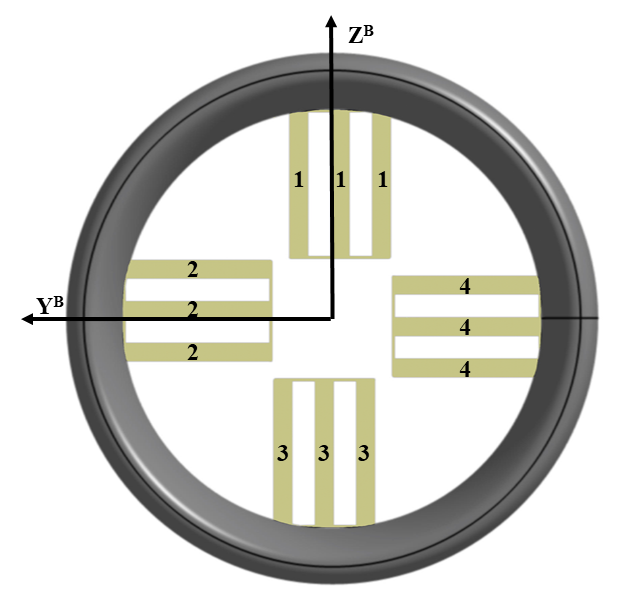
\includegraphics[width=0.3\textwidth]{vanes.png}
    \caption{\label{fig:control_vanes}操纵舵面示意图}
\end{figure}
\subsection{操纵舵面动力学}
操作舵面由四组相互独立的舵面及相应平行的导流板组成,其中1,3号舵面产生偏航力矩,2,4号舵面产生
俯仰力矩,所有舵面共同产生滚转力矩,如\autoref{fig:control_vanes}所示。本文中用$\delta_{1}$, $\delta_{2}$, $\delta_{3}$, $\delta_{4}$来
表示对应舵面组的偏转角度,最大偏转角度为30度。
由于控制舵面暴露在螺旋浆所产生的下洗流中。因此,由于每个导流板可以视为一片机翼,因此,其表面动压可以被建模为:
\begin{align}
    q_{cs}=\frac{1}{2} \rho_{\infty}\left(u-u_{wind}+v_{i}\right)^{2}
\end{align}
当使用四组操纵舵面去控制无人机的姿态运动时,控制量是冗余的。
因此本章采取了一种简单直接的控制分配方式\cite{zhang2013new}, 考虑下面的约束:
\begin{align}
    \delta_{1} = -\delta_{3}
\end{align}
控制分配形式如下:
\begin{align}
    \left[\begin{array}{l}
    \delta_{1} \\
    \delta_{2} \\
    \delta_{3} \\
    \delta_{4}
    \end{array}\right] & = \left[\begin{array}{ccc}
    0 & 0 & 0.5 \\
    0.5 & 0.5 & 0 \\
    0 & 0 & -0.5 \\
    0.5 & -0.5 & 0
    \end{array}\right]\left[\begin{array}{l}
    \delta_{x} \\
    \delta_{y} \\
    \delta_{z}
    \end{array}\right]
\end{align}
也就是说,控制系统将会根据姿态的误差输出相应的虚拟控制舵面$\delta_{x}$、$\delta_{y}$和$\delta_{z}$,
再经过控制分配得到实际的操纵舵面偏转量。因此,由于控制分配并非论文的重点,本文中后续使用的舵面偏转量实际上
是虚拟控制舵面所对应的偏转角度。
由操纵面产生的作用于机体的力和力矩可分别表示为:
\begin{align}
   \mathbf{F}_{\mathrm{cs}} & = q_{\mathrm{cs}} S_{\mathrm{v}} C_{\mathrm{L,v}}\left[\begin{array}{c}
    0\\
    -\delta_{z}  \\
    \delta_{y} 
    \end{array}\right] \\
    \mathbf{M}_{\mathrm{cs}} & = q_{\mathrm{cs}} S_{\mathrm{cs}} C_{\mathrm{L,v}}\left[\begin{array}{ccc}
    l_{1} & 0 & 0 \\
    0 & l_{2} & 0 \\
    0 & 0 & l_{2}
    \end{array}\right]\left[\begin{array}{c}
    \delta_{x} \\
    \delta_{y} \\
    \delta_{z}
    \end{array}\right]
\end{align}
其中,$C_{L,v}$表示舵面所对应的翼型的升力曲线斜率,$S_{v}$表示舵面的面积,$l_{1}$是相对于滚转轴的力臂,
$l_{2}$表示相对于俯仰/偏航轴的力臂。

\subsection{机体动力学}
当计算无人机气动时,可以将机身,机翼以及涵道视为一整个升力体\cite{zhang2013new},其中,气动力和气动力矩主要受机翼的影响。
空速、攻角和侧滑角对于无人机的气动特性有重要的作用,因此,空速、攻角和侧滑角计算公式如下:
\begin{align}
    V_{a} & =\sqrt{u_{r}^{2}+v_{r}^{2}+w_{r}^{2}} \\
    \alpha & =\tan ^{-1}\left(\frac{w_{r}}{u_{r}}\right) \\
    \beta & =\sin ^{-1}\left(\frac{v_{r}}{V_{a}}\right),
\end{align}
其中,
\begin{align*}
    \left\{\begin{matrix}
        u_{r} = u-u_{\text {wind }}\\
        v_{r} = v-v_{\text {wind }}\\
        w_{r} = w-w_{\text {wind }}
       \end{matrix}\right.
\end{align*}
由于垂直起降无人机在过渡过程中主要发生在纵向平面,即$o_{b}x_{b}z_{b}$平面。因此下面分别分析无人机的纵向空气动力学与横向空气动力学,并进行建模:
\subsubsection{纵向空气动力学}
无人机纵向空气动力和力矩会导致机身$i_{b}-k_{b}$平面(又称为俯仰平面)上的运动,如\autoref{fig:longitudinal}所示。图中描述了升力、阻力
和俯仰力矩,
\begin{figure}[htbp]
    \centering
    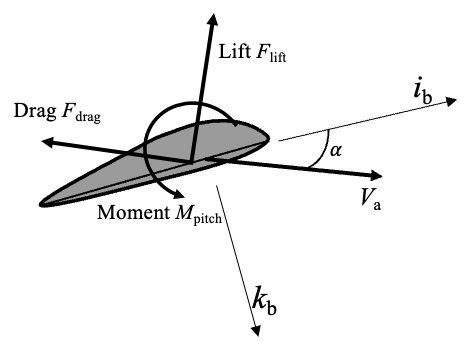
\includegraphics[width=0.5\textwidth]{airfoil.png}
    \caption{\label{fig:longitudinal}无人机纵向受空气动力分析}
\end{figure}
根据定义,升力、阻力以及俯仰力矩的变化很大程度上取决于空速与攻角,而在大部分文献中,为了简化模型,通常会基于低攻角假设,对升力、阻力以及俯仰
力矩进行一阶泰勒展开,这是因为,在典型的低攻角飞行条件下,流场在飞机机身上方为层流且附着在表面,空气将以有序的方式流过飞机表面,并不会发生分
离或湍流,这种流场通常被称为准稳态流场,这种流动的稳定性和可预测性意味着气动力和力矩相对于攻角的变化是平滑的,可以使用一阶泰勒近似。因此通常
在低攻角工作区域范围内,气动力和力矩可以采取线性模型进行建模\cite{kikumoto2022back},公式如下:
\begin{align}
    C_{L,n}(\alpha) &= C_{L_{0}}+C_{L_{\alpha}} \alpha \\
    C_{D,n}(\alpha) &=C_{D_{0}}+C_{D_{\alpha_{1}}} \alpha+C_{D_{\alpha_{2}}} \alpha^{2} \\
    C_{m,n}(\alpha) &= C_{m_{0}}+C_{m_{\alpha}} \alpha
\end{align}
其中,下标$n$表示此时处于低攻角工作区域,下标$L$表示对应的是升力系数,下标$D$表示对应的是阻力系数,下标$m$表示对应的是俯仰力矩系数。

而由于垂直起降无人机在垂直模态和水平模态的过渡转换过程通常位于高攻角工作区域\cite{argyle2016modeling},由此可能会诱发失速现象。作为一种最
重要的非稳态流动现象,失速通常指当攻角增加到气流与机翼分离的程度时,升力出现急剧下降的现象。这是因为在低攻角或中等攻角条件下,机翼上方的气流为
层流,并在流过机翼时附着在机翼上。而当攻角超过临界失速角时,气流开始从机翼顶面分离,造成湍流,机翼产生的升力因此骤减。所以在大攻角条件下,之前
的气动模型线性假设不再成立,而当飞机由于高攻角而产生失速现象时,机翼的作用可以被近似为一块平板\cite{stengel2005flight}。基于平板理论
\cite{kikumoto2022back,stengel2005flight,puopolo2013comparison,beard2012small},当攻角大于临界失速角时,气动模型可被如下表示:
\begin{align}
    C_{L,s}(\alpha) & =2 \operatorname{sign}(\alpha) \sin ^{2}(\alpha) \cos (\alpha) \\
    C_{D,s}(\alpha) & =2 \sin ^{2}(\alpha) \\
    C_{M,s}(\alpha) & =-\operatorname{sign}(\alpha) \sin (\alpha) \sin (\alpha / 2)
\end{align}
其中,下标$s$表示此时工作在高攻角区域。

通常如果希望获得在较大攻角范围内随攻角变化的高保真气动模型,需要进行大量的风洞试验以及详细的计算研究。因此,本文使用了一种基于混合函数的气动模型
,其可以适用于在较大攻角范围内($\alpha\in \left [ -180^\circ, 180^\circ\right ] $),并且可以很好的描述低攻角下的线性阶段和高攻角的失速现象,
同时为了考虑角速率对气动系数的影响,气动模型也进行了一定的修正,公式如下\cite{kikumoto2022back,beard2012small}:
\begin{align}
    C_{*} & = (1-\sigma(\alpha))C_{*,n}(\alpha)+\sigma(\alpha)C_{*,s}(\alpha) + C_{*_{q}}\frac{c}{2V_{a}}q
    \label{eq:aero}
\end{align}
其中,$*$表示下标可以是$L$,$D$和$m$,混合函数定义如下:
\begin{align}
    \sigma(\alpha) & = \frac{1+e^{-M\left(\alpha-\alpha_{s}\right)}+e^{M\left(\alpha+\alpha_{s}\right)}}{\left(1+e^{-M\left(\alpha-\alpha_{s}\right)}\right)\left(1+e^{M\left(\alpha+\alpha_{s}\right)}\right)}
\end{align}
\begin{figure}[htbp]
    \centering
    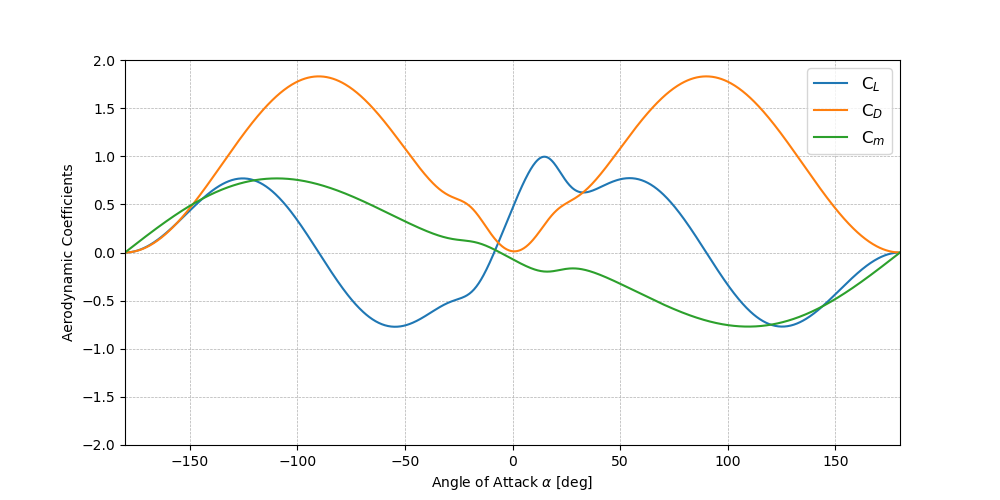
\includegraphics[width=0.8\textwidth]{aerocoeff.png}
    \caption{\label{fig:aerocoeff}无人机纵向受空气动力分析}
\end{figure}
基于上述公式,可以得到纵向气动系数随攻角变化的具体关系,如\autoref{fig:aerocoeff}所示。

由空气动力学可知,空气动力学的一般公式可以表示为:
\begin{align}
    L & =\frac{1}{2} \rho_{\infty} V_{a}^{2} S C_{L} \\
    D & =\frac{1}{2} \rho_{\infty} V_{a}^{2} S C_{D} \\
    m & =\frac{1}{2} \rho_{\infty} V_{a}^{2} S c C_{m}
\end{align}
其中,$C_{L},C_{D},C_{m}$由\autoref{eq:aero}计算,$L$表示升力, $D$表示阻力, $m$表示俯仰力矩,$S$表示机翼相对参考面积,c表示无人机的俯仰力臂.
\subsubsection{横向空气动力学}
无人机横向空气动力学包括由侧向力$Y$导致飞行器沿$j_{b}$轴的侧向平移运动以及受侧向力矩$l$和$n$影响的滚转和偏航运动。无人机横向空气动力学主要由
侧滑角$\beta$决定,同时还受滚转角速率$p$和偏航角速率$r$影响, 公式如下:
\begin{align}
    Y & = \frac{1}{2} \rho V_{a}^{2} S C_{Y}\left(\beta, p, r\right) \\
    l & = \frac{1}{2} \rho V_{a}^{2} S b C_{l}\left(\beta, p, r\right) \\
    n & = \frac{1}{2} \rho V_{a}^{2} S b C_{n}\left(\beta, p, r\right)
\end{align}
由于垂直起降无人机在过渡过程中横向运动的主要任务是保证稳定性,因此侧滑角的变化范围较小,可以基于一阶泰勒近似使用线性模型去描述其侧向空气动力学模型,公式如下:
\begin{align}
    C_{Y} & = C_{Y_{0}}+C_{Y_{\beta}} \beta+C_{Y_{p}} \frac{b}{2 V_{a}} p+C_{Y_{r}} \frac{b}{2 V_{a}}r\\
    C_{l} & = C_{l_{0}}+C_{l_{\beta}} \beta+C_{l_{p}} \frac{b}{2 V_{a}} p+C_{l_{r}} \frac{b}{2 V_{a}} r\\
    C_{n} & = C_{n_{0}}+C_{n_{\beta}} \beta+C_{n_{p}} \frac{b}{2 V_{a}} p+C_{n_{r}} \frac{b}{2 V_{a}} r
\end{align}

由于气动力$L,D,Y$定义在气流坐标系,因此需要结合\autoref{eq:Lab}进行坐标转换:
\begin{align}
    \mathbf{F}_{\text {aero}} & = L_{a}^{b}(\alpha ,\beta)\begin{bmatrix}
 -D\\
 -Y\\
-L
\end{bmatrix}\\
\mathbf{M}_{\text {aero}} & = \begin{bmatrix}
 l\\
 m\\
n
\end{bmatrix}
 \end{align}
\subsection{固定气动面动力学和陀螺力矩}
涵道无人机内部的固定气动面一般被设计用来平衡悬停状态下旋翼下的反扭力距。因此固定气动面对涵道轴的力矩可近似为:
\begin{align}
    \mathbf{M}_{f} & = \left[\begin{array}{lll}
    k_{f} (v_{i}+u_{r})^{2} & 0 & 0 
    \end{array}\right]^{T}
\end{align}
其中,$k_{f}$是固定舵面力矩系数。
通常情况下,陀螺力矩可以忽略不计,但当无人机执行诸如过渡等大角度机动时,陀螺力矩可能会变得很大。假设螺旋桨转速变化较小,则陀螺力矩可模拟为
\begin{align}
    \mathbf{M}_{\text {gyro }} & = n_{p} \omega_{p} J_{p}\left[\begin{array}{c}
    0 \\
    -r \\
    p
    \end{array}\right]
\end{align}
其中,$n_{p}$为转子个数,$J_{p}$为螺旋桨转动惯量,$p$和$r$是滚转和偏航角速率。

\section{强化学习概述}
\subsection{马尔可夫决策过程}
在强化学习中进行学习及实施决策的机器被称为智能体(agent),智能体之外的所有与其相互交互的事物都被称为环境,因此强化学习可以描述为这样一个与环
境交互的形式:智能体从环境中获得状态 (State,s) 输入,根据输入的状态选择动作(Action,a),环境根据智能体输出的动作呈现出新的状态($s^{'}$)并返回一个奖
励值 (Reward,r) 给智能体,如图所示。如果交互过程中,状态具备马尔可夫性,那么该过程可以被视为一个马尔可夫决策过程(Markov Decision Process,MDP),
通常由由$\left \langle S,A,P,\gamma,R \right \rangle$五元组构成。其中,$P$表示状态转移概率方程,$p\left(s^{\prime} \mid s, a\right)$
表达在状态s,动作a下过渡到新状态$s^{'}$;$\gamma$表示折扣因子,其反映了对当前奖励和未来奖励的权衡。$pi$通常表示智能体的策略,是状态映射到动作的
函数,其中,$\pi(a|s)$表示在状态$s$中选择动作$a$的概率。强化学习的任务被设定为最大化期望折扣回报,其中,折扣回报$G_{t}$为:
\begin{align}
    G_{t} = r_{t}+\gamma r_{t+1}+\gamma^{2} r_{t+2}+\gamma^{3} r_{t+3}+\ldots= \sum_{k = 0}^{\infty}\gamma^{k}r_{t+k+1} 
\end{align}
为了解决这一优化目标,强化学习引入了价值函数。值函数一般可以分为动作值函数和状态值函数,它们被用来评估智能体在给定状态(或给定状态与动作)下有多“好“
(由回报的期望值定义)。而回报的期望值取决于智能体每个状态下所选择的动作,即值函数的大小取决于智能体所采取的策略。
在策略$\pi$下状态$s$的价值函数被定义为:
\begin{align}
    V_{\pi}\left(s\right) & = \mathbb{E}_{\pi }\left[\sum_{k = 0}^{\infty} \gamma^{k} R_{t+k+1}\mid S_{t}= s\right]
\end{align}
类似地,策略$\pi$下在状态$s$时采取动作a的价值函数被定义为:
\begin{align}
    Q_{\pi}\left(s, a\right) =\mathbb{E}_{\pi }\left[\sum_{k = 0}^{\infty} \gamma^{k} R_{t+k+1}\mid S_{t}= s,A_{t}=a\right]
\end{align}

\subsection{强化学习算法介绍}
解决强化学习问题的方法通常可以分为两种:一是通过求解价值函数,并在此基础上进行策略优化的间接方法,即基于值函数的方法;另一种是通过参数化的策略表示,根据策
略梯度定理进行改进的直接方法,即基于策略的方法。
\begin{itemize}
    \item [1.] 基于值函数的方法\\
    基于值函数的方法的核心在于如何通过不断的环境探索来估计值函数,从而建立对整个状态-动作空间决策回报的度量,并以之做为决策的依据。常见的值函数估计方法包括:
    蒙特卡洛方法(MC)与时间差分算法(TD)。以动作值函数为例,MC算法通常会根据策略$\pi$进行采样,在回合结束后记录状态动作对$(s,a)$之后的累积期望回报,然后
    进行平均。而TD算法则无需等到回合结束,就可立即进行更新。最简单的TD(0)的更新方式为:
    \begin{align}
        V\left(S_{t}\right) \leftarrow V\left(S_{t}\right)+\alpha\left(R_{t+1}+\gamma V\left(S_{t+1}\right)-V\left(S_{t}\right)\right)
    \end{align}
    同时由于TD(0)只使用了单步信息进行更新,其方差相较于MC算法偏低。因此其思想被强化学习算法广泛应用,其中,最经典的当属Q-learning算法。
    Q-Learning的目标是估计动作价值函数Q,即在状态s下采取动作a的期望回报。这通过以下更新规则实现:
    \begin{align}
        Q\left(s_{t}, a_{t}\right) \leftarrow Q\left(s_{t}, a_{t}\right)+\alpha\left[r_{t+1}+\gamma \max _{a^{\prime}} Q\left(s_{t+1}, a^{\prime}\right)-\right. 
        \left.Q\left(s_{t}, a_{t}\right)\right]
    \end{align}
    深度Q网络(DQN)是一种经典的值函数方法,比较适用于离散动作空间。它扩展了Q-Learning,引入了深度神经网络来近似Q函数,使之能够处理高维输入,
    有效缓解了维度爆炸问题。
    DQN的关键创新在于:1.DQN引入了经验回放池存放智能体的MDP五元组,而在网络训练时,将会从经验池随机抽取样本,可以打破样本之间的相关性,稳定学
    习过程;2. DQN使用了两个网络,一个是不断更新的网络,另一个是更新频率较低的目标网络,这种软更新的技巧这有助于稳定学习过程,因为使用相同网络
    会导致样本的预测值一直在变化难以学习。
    \item [2.] 基于策略的方法\\
    值函数方法通过先求取价值函数,从而在此基础上进行策略迭代完成优化,因而最终策略的好坏很大程度上取决于价值函数是否准确。另外,在连续动作空间
    中, 动作价值函数遭遇到“维数灾难”,无法求得全部“状态-动作”对的价值。而基于策略的方法则没有这样的局限性。实际上,策略本身即为一个状态到动作
    的概率分布,从而可以通过参数化概率分布的方式,在给定分布框架的条件下求取其特定的参数。若用$\sigma$代表策略网络参数,则给定策略$\pi$可以表
    示为$\pi(a|s;\sigma)$或$\pi(\sigma)$。因此,基于策略梯度方法的最终目标转换成求取分布的最优参数的问题。策略梯度g如下所示:
    \begin{align}
        g & = \mathbb{E}\left[\sum_{t = 0}^{\infty} \Psi_{t} \nabla_{\sigma} \log \pi_{\sigma}\left(a_{t} \mid s_{t}\right)\right]
    \end{align}
    在最直接的Reinforce算法中,$\Psi_{t}$被设为$\sum_{t=0}^{\infty} r_{t}$,在策略参数更新时,reinforce会使用具有单条轨迹的蒙特卡洛采样来估计策略梯度,
    因此它也具有MC算法的方差大与无法即时更新的缺点。
    在此基础上,Actor-Critic框架被提出,其中 Actor 负责进行学习参数化策略,以提供智能体进行动作决策的功能; Critic负责学习价值函数,用来评估特定状态下的价值。
    这种框架的直接动机是:学习值函数通常比回报的蒙特卡洛估计具有更低的方差,同时也可能提供更加丰富的信息。在实际使用中,通常使用动作值函数或者优势函数来进行估计。
    
    当$\Psi_{t}$取$Q^{\pi}\left(s_{t}, a_{t}\right)$时,经典的算法包括DDPG与SAC。深度确定性策略梯度(DDPG)算法是一种结合了Actor-Critic架构和DQN的算法,
    适用于连续动作空间。DDPG的重要特性包括:1. 引入高斯噪声加大探索力度,DDPG中Actor网络直接输出动作的大小,缺乏对其他动作空间的探索,因此DDPG会对输出的动作加入
    高斯噪声以提升探索度。2.借鉴了DQN中的软更新技巧,极大稳定了学习过程。 而SAC算法则基于DDPG在策略优化中加入熵这一正则项来鼓励更多的探索,其重要特性包括:1.向
    传统的Q函数中加入策略的熵,即希望在满足最大化回报的同时最大化熵,而策略优化时,将最小化旧策略与以Q值作为能量的玻尔兹曼分布的KL散度。2. 自动调节温度系数:通过
    设定熵的上限,将原问题视为带约束优化问题,通过类似拉格朗日乘子法,完成温度参数的自动调节。3. 采用双Q网络减轻Q值的过估计情况,同时类似DQN采用软更新技巧,稳定
    其学习过程。

    当$\Psi_{t}$取$A^{\pi}\left(s_{t}, a_{t}\right)=Q^{\pi}\left(s_{t}, a_{t}\right)-V^{\pi}\left(s_{t}\right)$时,其中$A^{\pi}\left(s_{t}, a_{t}\right)$被定义为优势值函数,
    它量化了一个动作相较于平均可用动作的好坏程度,目前主流算法的实践中大多数采用广义优势估计(GAE)来进行优势函数的近似,其中最经典的算法要属TRPO与PPO。
    信任区域策略优化(TRPO)是一种基于单调策略改进定理进行优化的方法。令J($\pi$)表示在策略$\pi$下的期望折扣回报,单调策略改进定理表达如下:
    \begin{align}
        J\left(\pi^{\prime}\right)-J(\pi) & =\mathbb{E}_{s_{0}}\left[V_{\pi^{\prime}}\left(s_{0}\right)\right]-\mathbb{E}_{s_{0}}\left[V_{\pi}\left(s_{0}\right)\right] \\
        & =\mathbb{E}_{\pi^{\prime}}\left[\sum_{t=0}^{\infty} \gamma^{t} r\left(s_{t}, a_{t}\right)\right]+\mathbb{E}_{\pi^{\prime}}\left[\sum_{t=0}^{\infty} \gamma^{t}\left(\gamma V_{\pi}\left(s_{t+1}\right)-V_{\pi}\left(s_{t}\right)\right)\right] \\
        & = \mathbb{E}_{\pi^{\prime}}\left[\sum_{t=0}^{\infty} \gamma^{t} A_{\pi}\left(s_{t}, a_{t}\right)\right]
    \end{align}
    其中,$\pi^{\prime}$表示新策略,$\pi$表示旧策略。通过优化新旧策略之差,可以保证策略单调改进。但由于无法利用尚未更新的新策略去收集样本从而求解问题,
    因此TRPO基于新旧策略分布差异较小的约束假设,进行了一定的近似:
    \begin{align}
        J\left(\pi^{\prime}\right)-J(\pi)
        & \approx \mathbb{E}_{\pi}\left[\sum_{t=0}^{\infty} A_{\pi}\left(s_{t}, a_{t}\right)\frac{\pi^{\prime}(a_{t}|s_{t})}{\pi(a_{t}|s_{t})} \right]
    \end{align}
    考虑优化上式中的带约束优化问题,TRPO对目标函数和约束进行了泰勒展开,从而进行求解。TRPO算法的重要特性包括:1. 其很大程度上可以保证策略的单调提升,给出了比较有力的
    性能保证。2. 由于泰勒近似会引入一定的误差,为了保证满足KL散度约束,TRPO增加了线性搜索环节,保证训练时可以单调提升的。
    而PPO(近端策略优化)则基于TRPO的思想对问题进行优化,由于TRPO算法在对KL散度约束进行泰勒近似时需要使用策略的海森矩阵增加了极大的运算复杂度,因此PPO通过优化经过裁剪的
    目标函数进行一阶优化,当策略更新偏离原始策略太多时,这个函数会对这些更新进行裁剪,以维护更新的稳定性相比于TRPO算法极大的加快了训练速度,由于裁剪掉的样本不能够产生梯度
    PPO算法也提供了一定的训练稳定性。
\end{itemize}
\subsection{约束强化学习介绍}
\section{本章小结}
本章建立了涵道风扇式无人机的数学模型并介绍了强化学习相关的基础知识。首先定义了描述无人机运动的坐标系及其转换,给出了其运动学方程和动力学方程,
通过对涵道风扇式无人机模块化,分别对无人机动力学方程中涉及的气动力和气动力矩进行分析,并给出了其完善的无人机六自由度数学模型,为后续的过渡控制策略设计奠定了基础。其次对强化学习进行了简单概述,
介绍了马尔科夫决策过程及相关概念定义,并对解决强化学习问题的基于值和基于策略的方法做了较为详细介绍。

\chapter{基于约束强化学习的纵向无人机逆过渡策略设计}
\section{引言}
众所周知,涵道风扇式垂直起降无人机具备两种典型的工作模态分别是:水平飞行模态(level flgiht)和垂直悬停模态(hover)。逆过渡(Back-transition)问题的目标主要是实现
由水平飞行模态转垂直悬停模态即(Level flight to Hover,LTH),也是被公认为难度最大的过渡过程。因此,本章首先对之前的无人机六自由度模型进行纵向解耦建立强化学习环境,
然后将会介绍一种基于SAC的涵道式固定翼垂直起降无人机过渡策略控制方案,在保证过渡任务成功完成的前提下同时最小化过渡时间与过渡过程中的高度变化,并针对传统强化学习在面对
多项奖励函数难以设计的缺点,采用约束值函数的方式对其进行改进,保证了过渡过程中的鲁棒性与最优性。最后将与总能量控制算法、最优控制、传统强化学习算法分别进行对比,验证所提方
法的有效性。
\section{无人机逆过渡强化学习环境搭建}
在这部分中,我们将对完整的六自由度模型进行横纵向解耦,只考虑纵向三自由度涵道无人机动力学模型,从优化角度描述逆过渡过程中的期望性能指标及约束,并给出
强化学习中的环境搭建。这种模型简化的假设是因为:
一、在涵道无人机的过渡阶段,主要的动态变化集中于纵向平面,其中空气动力的变化尤为显著,从而对纵向控制策略提出了更高的要求。相比之下,横向动力学比较简单,通常可以采用线性化处理来进行简化。
适当的模型简化假设允许我们专注于纵向的控制策略,以便构建和评估过渡策略\cite{cheng2022transition,li2020transition}。
二、对于强化学习训练而言,三自由度无人机模型相比于六自由度模型只有近乎一半的状态空间和动作空间,可以加快评估不同的奖励函数以及超参数设置的过程\cite{gaudet2020deep}。
\subsection{逆过渡问题描述}
\label{sec:transition_problem}
\begin{figure}[H]
    \begin{tabular}{c}
    \hspace{-6mm}{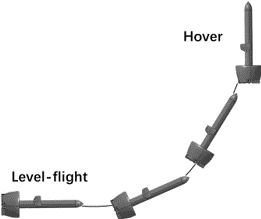
\includegraphics[height=5 cm,width=0.5\linewidth]{chapter3/CA.png}}\label{fig:CA}\\
    \hspace{-6mm}(\textbf{a}) 连续上升轨迹\\
    \hspace{-6mm}{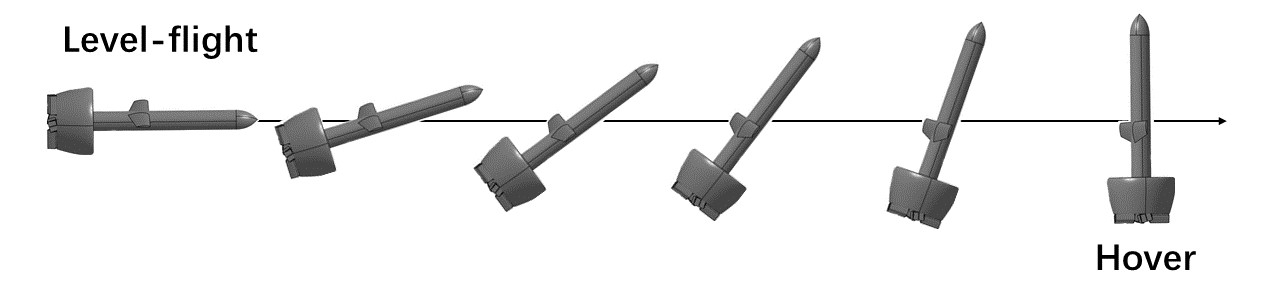
\includegraphics[width=1\linewidth]{chapter3/neat.jpg}}\label{fig:neat}\\
    \hspace{-6mm}(\textbf{b}) 整洁过渡
    \end{tabular}
    \caption{ 两种过渡方式.}
    \label{cmp} 
\end{figure}
一种简单且直接的逆过渡策略是让无人机以较大的俯仰角进行爬升\cite{green2005mav},将无人机水平飞行的动能转化为重力势能,从而减速完成过渡。例如:开源飞控“PX4”中的以恒定油门和阶跃俯仰角信号作为输入的线性
过渡轨迹和\cite{jeong2010transition}中提到的连续上升轨迹。这类过渡策略能够在短时间内完成,但通常伴随着显著的高度损失,如\autoref{fig:CA}。这不仅降低了无人机执行任务时的效率,尤其是在军事操作中,
还意味着无人机需要在过渡结束后耗费额外的能量和时间才能恢复至原定飞行高度。此外,由于悬停状态下的无人机需要更多能量来支撑自身重量,这进一步增加了整个过渡过程的能量消耗,进而影响了任务执行的整体效率。
因此在这种简单的方法基础上,“整洁过渡”,一种在过渡过程中高度不发生变化的过渡轨迹被提出\cite{cheng2022transition}, 如\autoref{fig:neat}。这种过渡方式通常意味着攻角会发生接近$90^{\circ}$的变化
,对控制器设计带来了困难。因此本文重点在于设计一个过渡策略在保证整齐过渡的前提下最小化过渡时间。下面给出该问题的数学形式:
基于无人机过渡变化主要发生纵向的假设,可以得到简化后的三自由度动力学方程为:
\begin{equation}
    \left\{
    \begin{aligned}
    \dot{u}&= g\sin \theta +\left (  D\cos \alpha -T-L\sin\alpha\right )/m -qw \\
    \dot{w}&= \left ( F_{d}+L\cos\alpha+D\sin\alpha +F_{cs} \right )/m+qu-g\cos\theta\\
    \dot{x}&= w\cos \theta-u\sin \theta \\
    \dot{z}&= u\cos \theta+w\sin \theta \\
    \dot{\theta}&=q\\
    \dot{q}&=\left ( m_{pitch} + M_{d} + M_{cs} \right ) /J_{y}
    \label{eq:three_dof}
    \end{aligned}
    \right.
\end{equation}
其中,无人机纵向状态量可以表示为:$X=\left [ u,w,\theta,q \right ]^{T}$, 控制量为:$U=[\omega _{p},\delta_{y}]$。因此对于\autoref{eq:three_dof}这样的动态系统,
期望最小化过渡时间:
\begin{align}
    J & = t_{f}
\end{align}
其中,$t_{f}$表示为终端时间,并考虑如下控制量约束和角速度约束:
\begin{align}
    \left\{\begin{matrix}
      \left | \delta _{y} \right |<30^{\circ}\\
        \omega _{pmin}<\omega _{p}<\omega _{pmax}\\
        \left | q \right |<90^{\circ}
    \end{matrix}\right.
\end{align}
其中,角速度约束主要是为了避免气动特性的显著变化。同时由于希望无人机在过渡过程中尽可能减小高度变化,实现"整洁过渡"\cite{cheng2022transition},考虑垂向速度约束:
\begin{align}
    &\left | V_{z} \right |<V_{z}^{m}
\end{align}
其中,$V_{z}^{m}>0$为固定常数,这样设计的原因是理想情况下,整洁过渡要求垂向速度$V_{z}$恒等于0,但实际飞行过程中,这样的等式约束往往难以满足,为此,可以对其等式约束
进行放宽转而变为小范围内的不等式约束。同时由于逆过渡过程要求无人机从水平飞行状态转换到垂直悬停状态,因此其初始条件和终端条件如下:
\begin{align}
    X_{t_{0}} &=\left [ V_{t_{0}}\cos \theta_{t_{0}},V_{t_{0}}\sin \theta_{t_{0}},\theta_{t_{0}},0 \right]^{T}\\
    X_{t_{f}} &=\left [ u_{t_{f}},w_{t_{f}},\theta_{t_{f}},q_{t_{f}}\right]^{T}
\end{align}
其中,$V_{t_{0}}$是初始水平飞行速度,其值通过初始角度$\theta_{t_{0}}$根基水平飞行模态配平求得,具体约束参数如\autoref{tab:constraints}所示。
\begin{table}[htbp]
    \caption{约束变量参数表}
    \label{tab:constraints}
    \begin{tabularx}{\linewidth}{@{}llX@{}}
        \toprule
        Variable & Description & Constraint \\
        \midrule
        \( \theta_{t_{0}} \) & 初始俯仰角 & [1°, 15°] \\
        \( V_{t_{0}} \) & 初始水平飞行速度 & [11.08, 15.74] \\
        \( \theta_{t_{f}} \) & 终端俯仰角 & [85°, 95°] \\
        \( u_{t_{f}} \) & 终端速度 & [0, 0.5] \\
        \( w_{t_{f}} \) & 终端速度 & [0, 0.5] \\
        \( q_{t_{f}} \) & 终端角速度 & [-5°, 5°] \\
        \( \omega _{p} \) & 螺旋桨转速(rpm) & [110, 8048] \\
        \( \delta _{y} \) & 舵面偏转角度 & [-30°, 30°] \\
        \( V_{z} \) & 垂向速度约束 & [-1,1] \\
        \bottomrule
    \end{tabularx}
\end{table}
\subsection{强化学习环境搭建}
强化学习中状态空间、动作空间设置如下:
\begin{equation}
    \begin{aligned}
    s &= \left(u,w,\sin \theta , \cos \theta , q, t_{left},\left | z \right | \right)^{T} \in R^{7}, \\
    a &= \left(\delta_{y},\omega_{r}\right)^{T} \in R^{2}.
    \end{aligned}
\end{equation}
其中,状态量包括在地面坐标系下的高度信息以及在机体坐标系下的速度和角度信息。角度的相关信息采用正余弦变换后的俯仰角去表征,这是因为正余
弦变换能够有效地编码方向信息,尤其是动力学中存在大量的旋转矩阵,同时正余弦变换还可以提供更稳定的数值属性。
$t_{left}$表示距离当前回合结束的剩余时间,这个特征的设计对于期望最小化过渡时间这一目标十分重要\cite{pardo2018time}。而动作空间选定为经过归一化后的
螺旋桨转速和舵面偏转,取值范围为[-1,1],当输出实际动作时,会根据动作的最大值和最小值进行放缩和平移。
奖励与成本函数设置如下:
\begin{gather}
    \Phi (s_{t})=k_{1}\sqrt{v_{x}^{2}+v_{z}^{2}}+k_{2}\left | \theta-\pi/2 \right | \\
    Reward=\kappa(\left | u \right | < 0.5 \ \text{and}\ \left | w \right | < 0.5\ \text{and}\ \left | \theta \right | < 5^{\circ}\ \text{and}\ \left | q \right | < 5^{\circ})+(\Phi (s_{t+1})-\Phi (s_{t}))\times (0.99)^{t/10}\\
    Cost=\mathbb I(\left | V_{z} \right |> 1 ) + \mathbb I(\left | q \right |> \pi/2  )  
\end{gather}
其中奖励与成本函数解释如下:
\begin{itemize}
    \item [1.] $\kappa$ 是对成功完成过渡的奖励,通常是一个较大的数值。这样的奖励函数从密度上比较稀疏(只有一步可以得到),给探索造成了很大难度,但可以提供很强的鲁棒性。
    成功过渡的定义同\autoref{tab:constraints}一样,需要满足终端状态量处于指定约束。
    \item [2.] $\Phi (s_{t})=k_{1}\sqrt{v_{x}^{2}+v_{z}^{2}}+k_{2}\left | \theta-\pi/2 \right |$是一种经典的奖励重塑(reward-shaping)形式,$Phi (s_{t})$
    在这里表示势能函数,可以将无人机朝期望目标状态引导,起到为智能体“导航”的作用,本质上是一种稠密奖励,起到辅助智能体的作用,
    其系数$(0.99)^{t/10}$有两层直观的物理意义:1. 它表示奖励函数会随着时间而逐步衰减符合我们期望时间最短的目标。2. 它表示随着离期望目标状态越近,辅助奖励所占据的比重
    越小,减小辅助奖励可能带来的负面影响。
\end{itemize}
环境状态转移设置如下:无人机环境状态转移可以由\autoref{eq:three_dof}中的动力学方程提供,同时为了精准描述环境状态转移,本文中一律采用四阶龙格库塔法进行仿真,
设无人机动力学模型为:$x_{t+1}=f\left(x_{t}, u_{t}\right)$,状态转移方程如下:
\begin{align}
    x_{t+1}&=x_{t}+\frac{\tau}{6}\left(k_{1}+2 k_{2}+2 k_{3}+k_{4}\right)\\
    k_{1} & =f\left(x_{t}, u_{t}\right) \\
    k_{2} & =f\left(x_{t}+\tau \frac{k_{1}}{2},u_{t}\right) \\
    k_{3} & =f\left(y_{n}+\tau \frac{k_{2}}{2}, u_{t}\right) \\
    k_{4} & =f\left(y_{n}+\tau k_{3}, u_{t}\right)
\end{align}
其中,$\tau$为仿真步长,取0.2s。根据上面这些设置,我们在$gym$中注册了我们的涵道无人机环境,以便后续强化学习算法的开发。
\section{基于RCRL的涵道无人机纵向逆过渡基本方案}


\section{基于总能量控制系统的逆过渡控制}
总能量控制系统(Total Energy Control System,简称TECS)是一种用于飞机飞行控制的系统。TECS的核心是通过控制无人机的俯仰角(升降舵)和油门,调整飞机的动能和势能的平衡。
这种方法可以在变化的飞行条件下通过调整动能和势能的变化,以达到期望的高度和速度,从能量角度出发处理了无人机飞行过程中高度和速度的耦合问题。
同时由于过渡过程中,传统的TECS控制方案难以适用于悬停状态,因此本文采用了一种改进的TECS控制系统\cite{argyle2016modeling}去执行涵道无人机的过渡控制,其基本控制原理和控制方案如下:
无人机在$z_{e}$轴上的能量变化主要来自于高度变化引发的重力势能变化以及垂向速度变化引起的动能变化,而在$x_{e}$轴上的能量变化来自于该轴上的速度变化。而无人机的油门通常可以
控制机体轴$x_{b}$上的能量变化,升降舵可以控制无人机的俯仰角间接的去控制机体轴$z_{b}$上的能量变化。因此,将能量误差分解为沿机体轴的分量可以得到\cite{argyle2016modeling}:
\begin{align}
    \tilde{E}_{x}=\left(\mathrm{m} g\left(h^{d}-h\right)+\frac{1}{2} \mathrm{~m}\left(\dot{h}^{d}\left|\dot{h}^{d}\right|-\dot{h}|\dot{h}|\right)\right) \sin (\theta)+\frac{1}{2} \mathrm{~m}\left(\dot{x}^{d}\left|\dot{x}^{d}\right|-\dot{x}|\dot{x}|\right) \cos (\theta) \\
    \tilde{E}_{z}=\left(\mathrm{m} g\left(h^{d}-h\right)+\frac{1}{2} \mathrm{~m}\left(\dot{h}^{d}\left|\dot{h}^{d}\right|-\dot{h}|\dot{h}|\right)\right) \cos (\theta)+\frac{1}{2} \mathrm{~m}\left(\dot{x}^{d}\left|\dot{x}^{d}\right|-\dot{x}|\dot{x}|\right) \sin (\theta)
\end{align}
其中,角标$_{d}$表示期望的,通常会根据经验先验给出。$h$表示无人机垂向高度,$\dot{x}$表示无人机水平飞行速度。由于动能误差的定义并未考虑方向,因此上述公式对动能误差的计算进行
了一定的修正。
根据机体轴上的能量误差,可以设计比例-积分-微分控制器(PID)为:
\begin{align}
    T_{c} & = k_{p, x} \tilde{E}_{x}-k_{d, x} \dot{\tilde{E}}_{x}+k_{i, x} \int_{t_{0}}^{t} \tilde{E}_{x} \mathrm{d}t \\
    \theta^{c} & = k_{p, z} \tilde{E}_{z}-k_{d, z} \dot{\tilde{E}}_{z}+k_{i, z} \int_{t_{0}}^{t} \tilde{E}_{z} \mathrm{d}t
\end{align}
其中,$\delta_{t}$为油门指令,$\theta^{c}$为控制器解算出的期望俯仰角。而在实际使用中,底层的控制信号应该是螺旋桨转速$\omega_{p}$以及舵面偏转$\delta_{y}$,因此还需要
设定控制律去进行底层的油门控制和姿态控制。对俯仰角采用串级PID控制律:
\begin{align}
    q^{c} & = k_{p, \theta}\left(\theta^{c}-\theta\right)-k_{d, \theta} \dot{\theta} +k_{i, \theta} \int_{t_{0}}^{t}\left(\theta^{c}-\theta\right) \mathrm{d}t\\
    \delta_{y}&= k_{p, q}\left(q^{c}-q\right)-k_{d, q} \dot{q} +k_{i, q} \int_{t_{0}}^{t}\left(q^{c}-q\right) \mathrm{d}t
\end{align}
对于油门控制,由于非线性耦合代数方程组(2-3)-(2-6)并不存在解析解,因此我们很难直接得到推力到螺旋桨转速的直接映射,因此我们对推力公式进行一定的假设:
\begin{align}
    T & = k_{1} \omega_{p}^{2}-k_{2} V_{a}^{2}
\end{align}
式中$\omega_{p}$表示螺旋浆转速,$V_{a}$表示空速,$k_{1},k_{2}$可以通过参数拟合求得,需要注意的是上述推力的公式建模并不准确,但是其建模误差可以很好的通过TECS控制
律进行补偿\cite{argyle2016modeling}。
根据上述公式,我们可以设计总能量控制系统去控制无人机,对于水平飞行转垂直悬停(LTH)的逆过渡过程,本文选择的速度参考曲线为初始值为$V=11 m/s$,加速度$a=-1 m/s^{2}$,
控制效果如下所示:

\section{基于伪谱法的无人机逆过渡轨迹优化}
% 由\autoref{sec:transition_problem}可知,无人机逆过渡轨迹优化问题也可采用最优控制算法进行求解。因此本文采用求解器GPOPS\cite{patterson2014gpops}进行求解,它
% 使用自适应\text{Radau}伪谱法,采用\text{Legendre-Gauss-Radau}点为离散配点,基于MATLAB平台实现。



\section{仿真结果对比与分析}

\section{本章总结}

%\chapter{}
% \section{强化学习环境搭建}
% \subsection{无人机过渡问题表述}
% 涵道风扇式垂直起降无人机具备两种典型的工作模态分别是:水平飞行模态(level flgiht)和垂直悬停模态(hover)。过渡问题的目标主要是实现两种工作模态之间的转换,在完成过渡转换的
% 基础上,过渡过程中的性能表现也是值得被关注的,例如:过渡转换时间,过渡过程高度变化,过渡过程飞行距离等。传统的过渡控制策略通常要求在先验给出参考过渡轨迹的条件下再去设计
% 控制器去进行跟踪。轨迹优化则通过直接法或间接法去求解一个最优控制问题来求解相应的过渡控制策略。
% 无人机过渡最优控制问题定义如下:
% 纵向平面内无人机动力学方程如下:
% \begin{equation}
%     \left\{
%     \begin{aligned}
%     \dot{u}&= g\sin \theta +\left (  D\cos \alpha -T-L\sin\alpha\right )/m -qw \\
%     \dot{w}&= \left ( F_{d}+L\cos\alpha+D\sin\alpha +F_{cs} \right )/m+qu-g\cos\theta\\
%     \dot{x}&= w\cos \theta-u\sin \theta \\
%     \dot{z}&= u\cos \theta+w\sin \theta \\
%     \dot{\theta}&=q\\
%     \dot{q}&=\left ( m + M_{d} + M_{cs} \right ) /I_{yy}
%     \end{aligned}
%     \right.
% \end{equation}
% 状态量$X=\left [ u,w,\theta,q \right ]^{T}$, 控制量$a=[\omega _{p},\delta_{y}]$, ,其中初始状态定义为$X_{t_{0}}$,终端状态定义为$X_{t_{f}}$。
% 要求满足下列约束的同时使性能指标最小:
% \begin{eqnarray}
%     J=t_{f}
% \end{eqnarray}
% \emph{\hl{s.t.}}
% \begin{enumerate}
% \item 角速率约束 $q<180^{\circ}$

% \item 控制量约束: $\left | \delta _{y} \right |<30^{\circ}$ and $\omega _{rmin}<\omega _{r}<\omega _{rmax}$

% \item 整洁过渡约束: $\left \| v_{z} \right \| < 1$\ m/s

% \item 无人机纵向动力学方程
% \end{enumerate}
% 而无人机的悬停状态为$X_{hover}=\left [ 0,0,90 ^{\circ},0\right ]^{T}$,水平飞行状态$X_{level flight} = \left [ V_{level}\cos (\theta),V_{level}\sin (\theta ),\theta,0\right ]^{T}$
% ,水平飞行状态可以根据初始俯仰角使用scipy.optimize中优化算法进行配平求得,其初始范围是$\theta\in \left [ 1^{\circ},15^{\circ} \right ], V_{level flight}\in \left [ 15.74 m/s, 11.08 m/s \right ]$
% 如果是从垂直悬停模态转水平飞行模态(HTL)的过渡过程,初始状态$X_{t_{0}}=X_{hover}$, 终端状态$X_{t_{f}}=X_{level flight}$;
% 如果是从水平飞行模态转垂直悬停模态(LTH)的逆过渡过程,初始状态$X_{t_{0}}=X_{level flight}$, 终端状态$X_{t_{f}}=X_{hover}$。




% 而强化学习则可以使用免模型算法在无需先验知识的条件下针对马尔科夫决策过程使用基于贝尔曼方程的
% \par 如\autoref{alg:sample},这是一个算法

% \begin{algorithm}[H]
%     \begin{algorithmic} % enter the algorithmic environment
%         \REQUIRE $n \geq 0 \vee x \neq 0$
%         \ENSURE $y = x^n$
%         \STATE $y \Leftarrow 1$
%         \IF{$n < 0$}
%             \STATE $X \Leftarrow 1 / x$
%             \STATE $N \Leftarrow -n$
%         \ELSE
%             \STATE $X \Leftarrow x$
%             \STATE $N \Leftarrow n$
%         \ENDIF
%         \WHILE{$N \neq 0$}
%             \IF{$N$ is even}
%                 \STATE $X \Leftarrow X \times X$
%                 \STATE $N \Leftarrow N / 2$
%             \ELSE[$N$ is odd]
%                 \STATE $y \Leftarrow y \times X$
%                 \STATE $N \Leftarrow N - 1$
%             \ENDIF
%         \ENDWHILE
%     \end{algorithmic}
%     \caption{\label{alg:sample}算法样例}
% \end{algorithm}